% !TEX root = memoire.tex
% !BIB program = biber

\chapter{Contexte et état de l'art : classification documentaire, indexation matière et intelligence artificielle}
\label{chap:partie1}

\section{La classification \textit{Library of Congress}}
\label{sec:lcc-histoire}

La classification de la Bibliothèque du Congrès, ou \textit{Library of Congress Classification} (LCC), a été mise au point en 1897 par James C. M. Hanson, responsable du service des catalogues de la \textit{Library of Congress}, avec la participation de Charles Martel\footcite[p.~19-21]{chan1990}. C'est un projet qui répondait à un besoin pratique de classification universelle du savoir, avec pour but principal d'organiser physiquement les collections de la plus grande bibliothèque des États-Unis et de construire un système d'inventaire réel des fonds, plutôt qu'une théorie préétablie des disciplines. Cette genèse s'inspire de la \textit{Dewey Decimal Classification} (DDC), conçue vingt ans plus tôt par Melvil Dewey, tout en s'en distinguant fondamentalement\footcite[p.~20]{chan1990}.

La DDC a une architecture récursive en dix classes. Elle a été conçue pour couvrir de façon homogène l'ensemble des savoirs avec une grande rigidité. La \gls{lcc},  a été construite classe par classe, au fil de l'inventaire réel des collections de la \textit{Library of Congress}.

Certaines classes, comme Bibliographie et sciences de l'information (Z) ou Langue et littérature (P), sont divisées en branches très diverses ; d'autres restent plus restreintes, selon le volume des collections concernées. La LCC a un trait structurel propre, qui est sans équivalent dans la \gls{ddc} : plusieurs lettres de l'alphabet n'ont encore aucune classe disciplinaire\footcite{tacq2006}. Cette absence d'affectation dans l'espace des notations possibles est différente du principe de la DDC. Elle permet de laisser de la place dans l'architecture d'ensemble pour accueillir de nouveaux développements disciplinaires.

Dans sa structure, la LCC repose sur 21 grandes classes désignées par une lettre majuscule de A à Z\footcite[p.~38-41]{chan1990}. Chaque classe va être subdivisée en “sous grande-classe", identifiée par une seconde ou une troisième lettre, elles-mêmes divisées en sous-sous-classes désignées par une plage numérique qui précise le sujet avec un degré de précision croissant. Cette structure s'articule ainsi autour de trois niveaux de nature différente : un niveau disciplinaire (la grande classe), un niveau thématique (la sous-classe et son intervalle numérique) et un niveau bibliographique individuel (le cutter).

\begin{figure}[h]
\centering
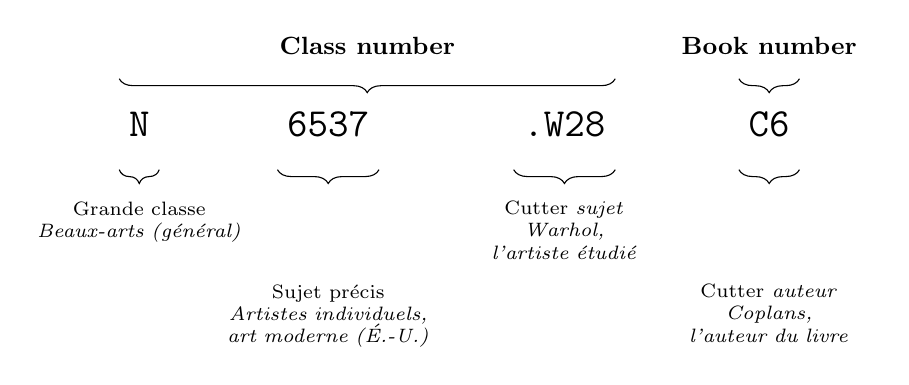
\begin{tikzpicture}[
    seg/.style={font=\ttfamily\Large, minimum height=1cm},
    lbl/.style={font=\scriptsize, align=center, text width=2.6cm},
    brace/.style={decorate, decoration={brace, amplitude=5pt, mirror}},
]
\node[seg] (n)    at (0,0)    {N};
\node[seg] (n6537) at (2.4,0) {6537};
\node[seg] (w28)  at (5.4,0)  {.W28};
\node[seg] (c6)   at (8.0,0)  {C6};

\draw[brace] ([yshift=2pt]n.north west) -- ([yshift=2pt]w28.north east)
    node[midway, yshift=12pt, font=\small\bfseries] {Class number};
\draw[brace] ([yshift=2pt]c6.north west) -- ([yshift=2pt]c6.north east)
    node[midway, yshift=12pt, font=\small\bfseries] {Book number};

\draw[brace] ([yshift=-2pt]n.south west) -- ([yshift=-2pt]n.south east)
    node[midway, yshift=-8pt, anchor=north, lbl] {Grande classe\\\textit{Beaux-arts (général)}};
\draw[brace] ([yshift=-2pt]n6537.south west) -- ([yshift=-2pt]n6537.south east)
    node[midway, yshift=-38pt, anchor=north, lbl] {Sujet précis\\\textit{Artistes individuels, art moderne (É.-U.)}};
\draw[brace] ([yshift=-2pt]w28.south west) -- ([yshift=-2pt]w28.south east)
    node[midway, yshift=-8pt, anchor=north, lbl] {Cutter \emph{sujet}\\\textit{Warhol, l'artiste étudié}};
\draw[brace] ([yshift=-2pt]c6.south west) -- ([yshift=-2pt]c6.south east)
    node[midway, yshift=-38pt, anchor=north, lbl] {Cutter \emph{auteur}\\\textit{Coplans, l'auteur du livre}};
\end{tikzpicture}
\caption{Anatomie d'une cote de rangement LCC en Classe N (Beaux-Arts) : Coplans, John, \textit{Andy Warhol}, classé N6537.W28 C6\footcite[p.~210-211]{chan1990}. Ce cas illustre la distinction entre le cutter \emph{sujet} (l'artiste étudié) et le cutter \emph{auteur} (le rédacteur de l'ouvrage).}
\label{fig:anatomie-cote-lcc}
\end{figure}

Un cutter est un code alphanumérique dérivé du nom d'auteur, du titre ou d'une zone géographique, qui permet de distinguer et d'ordonner alphabétiquement les documents partageant la même sous-classe\footcite[p.~80-88]{chan1990}.

La LCC se distingue enfin de la DDC par sa structure hiérarchique : les plages numériques ne rendent pas toujours explicites les relations entre les sujets voisins, à la différence de la logique strictement décimale de la DDC, qui permet de déduire une relation de proximité thématique directement dans la proximité numérique\footcite{tacq2006}. Mais de nombreuses classes de la LCC sont composées de plages non affectées, ce qui permet d'insérer de nouveaux sujets sans reconfigurer l'ensemble du système\footcite[p.~82]{chan1990}. Cette plasticité explique pourquoi la LCC, plutôt que la DDC, a été choisie comme référentiel par de grandes bibliothèques de recherche nord-américaines. Un choix effectué dans un contexte documentaire dont la problématique est de gérer des collections massives et en constante évolution sans risquer la saturation de la cotation.


Utilisée comme outil d'\textbf{indexation}, la LCC sert uniquement à décrire le sujet d'un document pour faciliter sa recherche. Utilisée comme \textbf{cote}, en revanche, elle détermine directement le rangement physique de l'exemplaire.
Dans ce mémoire, la deuxième fonction est celle qu'on utilise c'est à dire localiser physiquement un ouvrage en rayon à partir de sa cote. 

\subsection{La cote dans la notice bibliographique}
\label{sec:lcc-notice}

On distingue deux niveaux de description bibliographique : La notice bibliographique qui décrit l'œuvre en elle-même (titre, auteur, édition). La notice d'exemplaire (ou « partie d'exemplaire »),elle, décrit un exemplaire physique précis : son état matériel, son identifiant propre, et sa localisation en rayon. La cote décrite dans ce mémoire désigne l'endroit ou un exemplaire précis est physiquement rangé.

Le numéro de \gls{cutter}, dernière partie de la cote avant la date de publication, sert à distinguer et à ordonner alphabétiquement dans la même sous classe les éléments qui la partagent. La LCC repose pour cela sur un tableau de conversion propre, à un ou deux chiffres\footcite[p.~83]{chan1990}. Ce choix résout à la fois les contraintes d'espace sur la cote physique des ouvrages, mais aussi le problème des auteurs partageant les mêmes premières lettres.

La LCC ne constitue pas pour autant un référentiel figé.La \textit{Library of Congress} publie régulièrement des additions, modifications et le système continue d'évoluer au fil de l'apparition de nouveaux champs disciplinaires\footcite{tacq2006}. Cette adaptation continue est à prendre en compte lors du développement de la gestion d'un catalogue de bibliothèque.

La LCC détermine la position du document au sein d'une hiérarchie disciplinaire, mais elle ne dit presque rien sur le contenu intellectuel de ce document. Deux ouvrages classés dans la même sous-classe peuvent porter sur des sujets très différents. Cette fonction complémentaire relève d'un langage d'indexation matière. C'est l'objet de la section suivante, qui constitue également l'une des sources de données exploitées par le \textit{pipeline} dans sa proposition de sous-classe au \gls{llm}.


\section{RAMEAU et l'indexation matière en France}
\label{sec:rameau}

Si la LCC permet de ranger physiquement les documents selon les grandes disciplines, elle ne permet pas une indexation fine de leur contenu intellectuel. En France, cette fonction complémentaire d'indexation est assurée par un langage appelé RAMEAU. 

\subsection{Structure et principes du langage RAMEAU}
\label{sec:rameau-structure}

RAMEAU, Répertoire d'autorité-matière encyclopédique et alphabétique unifié, est le langage d'indexation matière adopté par les bibliothèques universitaires et de lecture publique françaises. 

Ce répertoire est développé et maintenu par le Centre national RAMEAU au sein de la Bibliothèque nationale de France, inspiré des \textit{Library of Congress Subject Headings} (LCSH), dont il reprend l'architecture générale tout en l'adaptant aux usages bibliographiques français\footcite{rameaubnf}. Les \gls{lcsh} (\textit{Library of Congress Subject Headings}) est le langage d'indexation matière de référence en anglais: elles couvrent l'ensemble des domaines de la connaissance selon une structure hiérarchique de vedettes principales et de subdivisions\footcite{locsubjectheadings}.

Une \gls{vedette-matiere} désigne en catalogage un terme ou une expression normalisée qui sert de point d'accès à une notice dans un catalogue. Une vedette matière décrit ainsi le \emph{sujet} d'un document de façon standardisée, ce qui permet de retrouver ensemble tous les documents portant sur un même sujet, même si leurs titres emploient des termes différents.


Concrètement, une vedette RAMEAU peut ainsi contenir une vedette thématique, une vedette de forme (précisant par exemple s'il s'agit d'un dictionnaire, d'un catalogue d'exposition ou d'un acte de congrès), ou encore une vedette chronologique ou géographique. Chaque élément est pris dans une liste contrôlée et combiné selon un ordre de préséance fixé par les règles d'application du langage\footcite{rameaubnf}. Le Fichier national des propositions RAMEAU (FNPR) rassemble plusieurs contributions d'établissements documentaires français, belges et suisses pour enrichir le vocabulaire en continuité avec les besoins d'indexation exprimés dans le réseau. RAMEAU est donc un projet collaboratif qui évolue en fonction des besoins de la communauté\footcite{rameauopendata}.

\subsection{Limites documentées du système}
\label{sec:rameau-limites}

Ce même fonctionnement syntaxique présente à la fois des avantages et des limites. Même si elle a l'avantage de proposer des chaînes de recherche organisées et lisibles pour l'utilisateur, elle soulève plusieurs critiques récurrentes de la part de la communauté professionnelle française. Michel Mingam, responsable du Centre national RAMEAU, dresse un bilan nuancé de ce langage durant son 25e anniversaire et souligne que la difficulté n'est pas dans la nature pré-coordonnée du langage, mais dans la complexité de sa syntaxe d'application, jugée peu intuitive pour les usagers\footcite{mingam2005}. 


Cela pose une limite plus spécifique à ce mémoire. RAMEAU, bien qu'inspiré des \gls{lcsh} américains, a largement évolué au fil des enrichissements successifs du réseau français par rapport à sa source originale\footcite[p.~41]{mingam2005}. Cette dérive entre les deux référentiels introduit une incertitude supplémentaire pour un traitement automatisé qui chercherait à établir une correspondance directe entre une vedette RAMEAU et son équivalent \gls{lcsh} théorique.


\subsection{Conséquences pour un traitement automatisé}
\label{sec:rameau-consequences}

Ces deux limites, la complexité syntaxique et la dérive terminologique par rapport aux \gls{lcsh}, ont des conséquences directes pour le traitement automatisé du champ sujet d'une notice bibliographique. Ce champ, qui contient les vedettes RAMEAU, constitue un objet thématique dont l'information est difficile à décomposer algorithmiquement d'une notice à l'autre. La richesse des vedettes est elle-même hétérogène : certaines notices sont riches en vedettes, d'autres beaucoup plus pauvres.

Cette difficulté prend une importance particulière dans le cadre présent de ce travail, où l'un des objectifs a été d'évaluer si le champ RAMEAU constitue une des sources d'enrichissement considérées pour l'automatisation. La question est de savoir si une vedette RAMEAU, en dépit de l'hétérogénéité des données, apporte au modèle de langage une information plus riche qu'un simple titre pour orienter sa proposition de sous-classe LCC. 

Au-delà de RAMEAU, le traitement automatisé doit aussi être adapté à la nature du fonds documentaire traité, notamment lorsque le corpus n'est pas généraliste mais spécialisé. C'est précisément le cas des bibliothèques patrimoniales et musées, dont les logiques de catalogage diffèrent de celles d'une bibliothèque de lecture publique ou universitaire.


\section{Bibliothèques patrimoniales et de musée, un terrain spécifique}
\label{sec:bibliotheques-patrimoniales}

\subsection{Spécificités documentaires des bibliothèques de musée et systèmes alternatifs}
\label{sec:bibliotheques-specificites}

Les bibliothèques rattachées à des institutions patrimoniales présentent, comparées aux bibliothèques généralistes ou universitaires, un profil documentaire spécifique. Elles possèdent une volumétrie généralement plus restreinte, de quelques dizaines à quelques centaines de milliers de documents, alors que les grandes bibliothèques universitaires en comptent souvent plusieurs centaines de milliers, parfois davantage, et leurs fonds présentent une cohérence thématique liée à leur institution patrimoniale, dont le périmètre scientifique, généralement plus spécialisé, détermine cette cohérence.


En Amérique du Nord, certaines bibliothèques d'art ont développé des systèmes de classification alternatifs plutôt que d'adapter directement des référentiels standardisés comme la LCC ou la DDC. C'est le cas de la \textit{Thomas J. Watson Library du Metropolitan Museum of Art}, dont la classification interne (la « MMA Classification »), fondée sur la \textit{Dewey Decimal Classification} (DDC) et les tables Cutter, a été publiée dès 1911 et conçue pour faciliter le repérage des ouvrages par le personnel curatorial plutôt que pour une logique d'accès standardisée\footcite{fultz2020}. Ce système, mis à jour à la main pendant près d'un siècle, n'a été abandonné qu'en 2002 au profit des cotes \textit{Library of Congress}, précisément pour accélérer le catalogage et permettre l'import de notices bibliographiques externes déjà pourvues d'une cote LC\footcite{fultz2020}. Certaines institutions s'inspirent d'une architecture standardisée existante (DDC ou LCC) et y ajoute des développements locaux adaptés à sa collection.

On retrouve cette dynamique, avec quelques nuances, à la bibliothèque du Musée d'Orsay. Rattachée à un établissement muséal, celle-ci présente un système de cotation interne, local, qui demande un changement de logique et d'adaptabilité lors de l'approche d'un déménagement et d'ouverture au public. 
L'équipe qui s'interoge sur le nouveau plan de cotation s'inspirent de la LCC. Elle sélectionne spécifiquement les branches d'intérêt pour les adapter aux collections. 

 
 Le reclassement étudié dans ce mémoire vise à optimiser la conversion de ce système local vers un référentiel standardisé, à l’occasion de l’ouverture de la bibliothèque au libre accès.
C'est cet écart entre l'exhaustivité de la LCC et la spécialisation du fonds qui motive l'hypothèse centrale de ce travail : vérifier si restreindre le périmètre de classification proposé au modèle de langage a un impact significatif sur la performance. 


\section{Intelligence artificielle et catalogage automatique, état de la recherche}
\label{sec:ia-catalogage}

\subsection{Premiers travaux d'automatisation de l'indexation matière}
\label{sec:ia-premiers-travaux}

La question de l'automatisation du catalogage et de la classification documentaire n'est pas nouvelle pour les sciences de l'information. Elle a longtemps mobilisé des approches fondées sur l'appariement de chaînes de caractères, le traitement automatique des langues par des méthodes diverses et plus récemment, l'apprentissage automatique supervisé au moyen de corpus annotés. 


\subsection{Approches récentes par grands modèles de langage (2024-2025)}
\label{sec:ia-llm-recentes}

Les travaux récents convergent en partie sur un constat, observé à plusieurs échelles et sur plusieurs référentiels : les LLMs obtiennent de bien meilleurs résultats sur les champs factuels et structurés d'une notice que sur ceux qui exigent un jugement sémantique fin, comme le choix d'une classe ou d'une vedette-matière.

Chow, Kao et Li (2024) mènent une expérimentation sur l'usage de ChatGPT pour l'attribution de vedettes LCSH à des thèses et mémoires électroniques\footcite{chow2024}. Dobreski et Hastings (2025) soumettent trois agents conversationnels grand public (ChatGPT, Gemini, Copilot) à un test portant simultanément sur l'attribution de cotes DDC, de cotes LCC et de vedettes LCSH ; leurs résultats indiquent une performance globalement faible, en particulier pour l'attribution de cotes, les erreurs les plus fréquentes consistant en des propositions trop générales ou portant sur un sujet erroné\footcite{dobreski2025}. Martins (2024), de son côté, teste la capacité de Claude (grand modèle de langage de l'entreprise Anthropic) à produire une cote complète, une vedette-matière et un numéro de cutter pour un même ouvrage, et conclut que l'outil peut alléger la charge de l'analyse documentaire sans pouvoir s'y substituer entièrement, notamment faute de constance dans ses réponses d'une session à l'autre\footcite{martins2024}.
 
Ces résultats  suggèrent que la difficulté observée tient à une limite plus générale des modèles de langage actuels face à la classification documentaire fine. 


\subsection{Approches few-shot et \textit{human-in-the-loop}}
\label{sec:ia-fewshot-hitl}

Au-delà de l'indexation matière, d'autres travaux montrent qu'il existe une même limite, mais à une autre échelle. Banerjee, Ingram et Fox (2024) étudient ainsi l'automatisation de la classification au niveau d'un chapitre plutôt que d'un document entier, pour des thèses et mémoires électroniques\footcite{banerjee2024}. Ils constatent la difficulté de produire une délimitation automatique des frontières thématiques internes à un document, et remarquent que même au niveau du chapitre, cette délimitation reste sujette à des erreurs. Quel que soit le référentiel choisi (LCSH, LCC, DDC) ou l'échelle de granularité étudiée (document entier ou chapitre), les travaux convergent vers un même constat : les études s'accordent très largement sur la nécessité d'associer une vérification humaine, aussi appelée \textit{human-in-the-loop} (HITL), plutôt qu'une automatisation non supervisée du catalogage.

Ce consensus constitue l'un des fondements du programme d'expérimentation mené par la \textit{Library of Congress}.

\section{Le cas de la \textit{Library of Congress} : son programme d'expérimentation }
\label{sec:lc-labs}

\subsection{Présentation du programme d'expérimentation}
\label{sec:lc-labs-presentation}

Au sein même de la \textit{Library of Congress}, une unité appelée \textit{LC Labs} a mené, dans le cadre d'un programme de plusieurs années, une expérimentation systématique sur l'apport des technologies d'intelligence artificielle aux processus de catalogage, appelée \textit{Exploring Computational Description} (ECD)\footcite{saccucci2025}.

Ce programme est composé de deux phases successives : une première phase (ECD~1) vise à tester plusieurs méthodes sur des données de livres numériques afin de calculer des seuils de performance de référence et d'obtenir une première compréhension des données disponibles. Une seconde phase (ECD~2) approfondit ce travail en se concentrant sur le prototypage du flux de travail d'assistance et sur la production de données au format MARC valide.

Le programme \textit{LC Labs} participe à une démarche de recherche appliquée guidée par deux buts fondamentaux : soutenir le travail du catalogueur professionnel sans le remplacer, tout en maintenant des exigences de qualité documentaire jugées non négociables au regard des standards établis de la description bibliographique.

Sur le plan méthodologique, la phase ECD~1 a testé plusieurs familles de modèles pour proposer automatiquement des champs de notice, des plus classiques aux modèles génératifs de la famille \gls{gpt}, toujours associés à une validation humaine. La phase ECD~2 a ensuite resserré le périmètre technique autour de modèles ouverts de la famille Mistral, avec une trentaine d'expérimentations visant à affiner la façon d'interroger le modèle (\textit{prompting}) et, dans certains cas, à le ré-entraîner sur des données spécifiques à la tâche (\gls{finetuning})\footcite{saccucci2025}.

Cette orientation méthodologique inspire directement le cadre d'évaluation de ce mémoire : le choix de concentrer une large part des expérimentations sur la famille Mistral est motivé par des considérations pratiques d'accès, tout en faisant écho aux pratiques expérimentales de la \textit{Library of Congress}.

\subsection{Résultats publiés et limites identifiées}
\label{sec:lc-labs-resultats}

Les résultats publiés par \textit{LC Labs} sont variés selon les modèles et la nature des champs bibliographiques concernés. Les scores varient fortement d'un modèle à l'autre : Mistral obtient les meilleurs résultats, avec une précision allant de 61~\% pour les sujets à 89,58~\% pour les genres, en passant par 80~\% pour le titre et 81,75~\% pour l'auteur principal\footcite{saccucci2025}.

La revue manuelle des suggestions de sujets produites par la recherche vectorielle lors de la phase ECD~2 indique que seules 42,9~\% des meilleures suggestions sont jugées acceptables par les experts, tandis que 29~\% sont jugées erronées, 22,5~\% trop larges et 5,6~\% trop étroites. Ces résultats sont obtenus sur un corpus généraliste de livres numériques, évalué selon un jugement humain binaire\footcite{saccucci2025}.

Les analyses détaillées des commentaires d'évaluation révèlent plusieurs typologies d'erreurs récurrentes : des ordres de subdivision incorrects, des sujets trop larges liés à l'absence d'une subdivision géographique nécessaire, des sujets trop étroits lorsque la subdivision géographique attendue n'est pas trouvée, ou encore des confusions de champs MARC lorsque la proposition ne couvre pas l'ensemble des lieux traités dans l'ouvrage.

Sur la base de ce diagnostic, les auteurs concluent que la performance des modèles testés ne permet pas d'envisager un fonctionnement pleinement automatique du catalogage. Ils préconisent une combinaison articulant assistance algorithmique et intervention humaine (\textit{human-in-the-loop} et \textit{AI-in-the-loop}), assortie de procédures d'assurance qualité et de normes explicites.

Ce rapport laisse ainsi plusieurs questions de recherche ouvertes, notamment sur la gestion des vedettes-matière post-coordonnées. A l'échelle d'une bibliothèque patrimoniale aux fonds spécialisé la question est de savoir si les résultats obtenus sont similaires et comment optimiser les modalités d'organisation de cette automatisation assistée.


\section{Fondamentaux techniques : \textit{few-shot prompting} et \textit{embeddings}}
\label{sec:fondamentaux-techniques}

\subsection{Le paradigme du \textit{few-shot prompting}}
\label{sec:fondamentaux-fewshot}

Une technique mobilisée dans ce mémoire est l'apprentissage en contexte (\textit{in-context learning}), popularisé par la démonstration des capacités du modèle GPT-3\footcite{brown2020}. Cela désigne la capacité d'un grand modèle de langage à adapter son comportement à une tâche donnée à partir de quelques exemples fournis directement dans les instructions (\textit{prompt}). C'est une méthode distincte de l'apprentissage supervisé classique, qui ne nécessite pas de ré-entraînement du modèle.

Le choix de la structure de l'instruction (\textit{prompt template}) ainsi que la sélection des exemples influencent de façon sensible les performances du LLM. Ils permettent d'orienter et d'optimiser ses réponses, plutôt que de s'en remettre à une sollicitation arbitraire.

Ces résultats sur le \textit{few-shot prompting} montrent que la performance du système ne dépend pas seulement des capacités générales du modèle employé, mais aussi de la pertinence et de la qualité des exemples choisis pour illustrer la tâche.

Cette approche est directement appliquée au plan de cotation de la bibliothèque du Musée d'Orsay : une sélection d'exemples pertinents, issue du corpus de référence, est intégrée pour guider le LLM dans l'attribution d'une cote.

\subsection{Représentations vectorielles et similarité sémantique}
\label{sec:fondamentaux-embeddings}

La sélection des exemples fournis en \textit{few-shot} repose elle-même sur une technique distincte. Les \textit{embeddings}, ou représentations vectorielles lient à des mots ou un ensemble de mots un vecteur numérique de grande dimension, construit de telle sorte que deux textes proches sur le plan sémantique soient représentés par des vecteurs proches dans cet espace. La proximité entre deux vecteurs se mesure  par la similarité cosinus qui compare l'orientation de deux vecteurs indépendamment de leur norme.
 
Cette technique permet, pour une notice donnée, de retrouver automatiquement les notices déjà cotées les plus proches dans un corpus de référence, sans reposer sur des de mots-clés. C'est un des éléments  \textit{few-shot} du \textit{pipeline} développé pour ce mémoire : les exemples présentés au LLM sont sélectionnés parmi les notices du corpus de référence dont le titre et les sujets sont les plus proches de la notice cible. 


\subsection{Paramètres de génération et déterminisme du modèle}
\label{sec:fondamentaux-temperature}

Au-delà de la formulation des instructions et du choix des exemples fournis en contexte, la performance du modèle sollicité dépend aussi des paramètres de génération utilisés. Parmi eux, la température qui contrôle le degré d'aléa introduit dans la sélection du prochain \textit{token}. Le \textit{token}  est l'unité minimale de traitement d'un modèle de langage (un mot, une partie de mot ou un caractère).

La température influe directement sur le comportement du modèle : une valeur élevée augmente la diversité et la créativité des réponses au détriment de la reproductibilité, tandis qu'une température proche de zéro contraint le modèle à choisir systématiquement les \textit{tokens} les plus probables, rendant la génération quasi déterministe.

Pour une tâche de classification à réponse contrainte, l'objectif ne réside pas dans la créativité ou la variété des formulations, mais dans la capacité à reproduire une décision de manière cohérente pour une entrée donnée. Le choix d'une température basse constitue donc une option méthodologique cohérente avec cet objectif.

Néanmoins, l'abaissement de la température n'élimine pas totalement la variabilité des réponses. Comme le souligne Martins (2024), même un modèle comme Claude ne produit pas toujours des réponses strictement identiques d'une session à l'autre pour une même requête de classification\footcite{martins2024} : une température minimale ne supprime pas l'aléa résiduel, mais permet d'en réduire significativement l'amplitude.

Ces choix de paramétrage ne suffisent cependant pas à éliminer certaines limites plus profondes, structurelles au fonctionnement même des grands modèles de langage.

\section{Limites connues des grands modèles de langage}
\label{sec:limites-llm}

La littérature scientifique a identifié et documenté un ensemble de limites structurelles qui conditionnent la conception de tout outil de production automatisée s'appuyant sur des LLM. Trois d'entre elles concernent directement la conception du pipeline présenté en Partie 2 de ce mémoire : l'hallucination, la nature statique des connaissances du modèle, et la sous-représentation des domaines spécialisés dans les données d'entraînement.

\subsection{Le phénomène d'hallucination}
\label{sec:limites-hallucination}

L'hallucination se définit comme la génération, par un modèle de langage, d'un contenu syntaxiquement correct et plausible, mais factuellement inexact ou non fondé sur des données vérifiables\footcite{ji2023}. Les synthèses de la littérature consacrées à ce phénomène mettent en évidence qu'il est possible d'en limiter l'ampleur par plusieurs leviers : des interventions en amont sur la qualité des données d'entraînement, des ajustements de l'architecture ou du processus d'entraînement du modèle, ou encore des contrôles et des vérifications en aval sur la sortie produite.


\subsection{Connaissances statiques et absence de vérification factuelle}
\label{sec:limites-connaissances-statiques}

Une autre limite documentée tient à la nature des connaissances du  modèle de langage. Un modèle de langage n'a pas accès à des sources d'information actualisées en l’absence de mécanisme de recherche externe. Ces connaissances proviennent de données fournies à son entraînement, sans mécanisme natif de vérification factuelle après coup. 


C'est une limite qui rejoint un champ de recherche plus large appelé conflit de connaissances (\textit{knowledge conflict}). Un conflit de connaissances survient lorsqu'une information fournie dans le contexte d'un modèle entre en tension avec la connaissance interne qu'il a acquise pendant son entraînement \footcite{xu2024}.  Les travaux sur ce phénomène montrent que les modèles de langage ont tendance à privilégier leur connaissance interne lorsque le contexte fourni est ambigu, de qualité inégale ou peu spécifique. En revanche, plus l’information contextuelle est pertinente et non ambiguë, plus le modèle aura tendance à s’appuyer sur elle plutôt que sur ses connaissances générales\footcite{xu2024}.

Cette observation a une implication pour la conception de l'architecture de l'outil de ce mémoire (voir \textref{chap:partie3}). Un modèle de langage sollicité pour proposer une cote a déjà une connaissance générale du système, vu qu'on a opté pour \textit{prompting} plutôt que \textit{fine-tuning}. Mais cette connaissance générale ne va pas forcément suivre les règles de politique documentaire propres à une institution particulière.

\subsection{Une limite additionnelle : la spécialisation documentaire }
\label{sec:limites-specialisation}

Une dernière limite, plus spécifique au terrain de ce mémoire, tient à la composition même des corpus sur lesquels les grands modèles de langage sont entraînés. Ces corpus, de très grande taille, sont construits à partir de données majoritairement issues du web généraliste, où la représentation des différents domaines de connaissance est fortement inégale.

Certains domaines bien structurés dans leur contexte professionnel n'occupent, à l'échelle d'un corpus web général, qu'une place marginale, un phénomène documenté dans la littérature sous le nom d'effet de « longue traîne »\footcite{kandpal2023,badhe2026}, détaillé en Partie 3 (\S\ref{sec:discussion-litterature}).

Ce cadre s'applique directement au terrain d'étude de ce mémoire : la bibliothèque du Musée d'Orsay est avant tout une bibliothèque spécialisée et de recherche, dont l'ultra-spécialisation chronologique et thématique, plus que son caractère patrimonial, façonne le fonds (arts décoratifs, histoire de l'art du dix-neuvième siècle, muséologie), des classes qui n'occupent, à l'échelle d'un corpus web généraliste, qu'une place marginale. Il y a donc un déséquilibre entre l'importance de ces classes dans le contexte documentaire local de la bibliothèque et les données d'entraînement du modèle sollicité.

